%!TeX root=../tese.tex
%(dica para o editor de texto: este arquivo é parte de um documento maior)
% para saber mais: https://tex.stackexchange.com/q/78101/183146

\chapter{Redes neurais no contexto de aprendizado de máquina}
\label{cap:redes}

Neste capítulo são apresentados alguns conceitos básicos de ciência de dados e de aprendizado de máquina, alguns dentre os vários tipos e exemplos de algoritmos de aprendizagem, direcionando-os para aquele que é o foco do trabalho, ou seja, as redes neurais artificiais.

Neste texto os termos ``algoritmo'' e ``técnica'' serão usados livremente como sinônimos, pois uma técnica de aprendizado de máquina, no contexto atual, é um algoritmo executado no computador que tem por objetivo ajustar parâmetros de modelos estatísticos.

Analogamente à definição dada na Introdução, citamos outras duas. Prince Barpaga \citep{prince} define aprendizado de máquina como sendo um ramo da inteligência artificial, em que computadores são treinados a partir de dados conhecidos para realizar alguma tarefa específica, ao invés de ser explicitamente programado para exibir uma resposta fixa.

Similarmente, Robbie Allen \citep{allen} descreve que um conjunto de dados é usado para ajustar um modelo estatístico de forma que, ao ser deparado com dados similares aos dados usados para o treino, saberá como tratá-los. Geralmente, conjuntos de dados e respostas ($x_i$'s e $y_i$'s) são usados como entradas para esses modelos, que a partir de novos dados ($x_j$'s), irão fornecer as predições de interesse ($\hat{y}_j$'s).

Concluindo, pode-se utilizar o grau de supervisão humana durante o aprendizado para separar os modelos em diferentes tipos, como é descrito por Géron \citep{hands}. Durante o aprendizado podem ser fornecidos um conjunto de consultas e de respostas já conhecidas. Tais respostas foram dadas por humanos, ao menos neste momento, e daí o termo ``supervisão humana''.

\section{Tipos de aprendizagem}

Um algoritmo de \defi{aprendizado supervisionado} é usado quando conhecemos características dos dados que estamos utilizando. De modo geral já temos de antemão as respostas às consultas para os dados utilizados no treinamento. Por exemplo, se estamos classificando fotos de animais, possuímos um conjunto de fotos para as quais já sabemos quais são de gatos, cachorros, etc.

O ato de rotular previamente os dados que usamos no treinamento é o que designamos de supervisão humana. Uma vez \emph{treinado}, o algoritmo recebe uma foto, ou seja, uma nova consulta e então fornece a resposta, neste caso se essa é a foto de um gato, ou cachorro, ou qualquer outra resposta dentre aquelas que foram dadas como exemplos durante o treinamento.

No escopo do aprendizado supervisionado citamos dois tipos principais de problemas. O primeiro é a \defi{classificação}, que é usada para rotular ou dividir os dados em classes pré-determinadas, a partir de exemplos, que é exatamente o caso dos exemplos descritos nos parágrafos anteriores, e ilustrada na Figura \ref{fig:classify}.

\begin{figure}[htb]
\centering
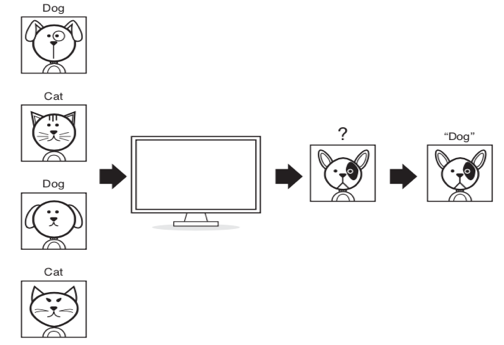
\includegraphics[width=7.5cm]{figuras/classificacao}
\caption{Tarefa de classificação de fotos de animais. As duas primeiras colunas ilustram o treinamento, e as duas últimas a previsão, de valores discretos, ou seja, ``classes''.\footnote{Extraído de \citep{allen}}}
\label{fig:classify}
\end{figure}

O segundo tipo de problema é a \defi{regressão}, usada para prever valores, ou seja, fornecer respostas a consultas ainda inéditas, sejam dados do futuro ou valores de funções em pontos do domínio para os quais ainda não existem valores. Podemos entender a diferença, com a ajuda de Allen \citep{allen} se percebermos que na classificação as respostas são valores discretos, isto é, um `cachorro' ou um `gato'. Enquanto isso na regressão, as respostas são valores contínuos, um intervalo real de possibilidades. Como exemplo, Allen \citep{allen} ilustra na Figura \ref{fig:regressao}, dado uma imagem radiológica, um modelo poderia prever em quantos anos uma pessoa poderia desenvolver alguma doença.

\begin{figure}[htb]
\centering
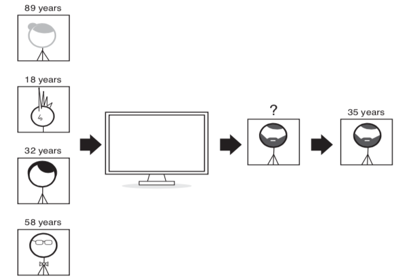
\includegraphics[width=7.5cm]{figuras/regressao}
\caption{Tarefa de regressão, mostrando novamente as fases de treinamento de de previsão, lidando com quantidades contínuas.\footnote{Extraído de \citep{allen}}}
\label{fig:regressao}
\end{figure}

Por outro lado, no \defi{aprendizado não-supervisionado} não sabemos os rótulos dos dados que estamos lidando, isto é, não sabemos previamente respostas aos dados conhecidos, assim o algoritmo deverá deduzir respostas de forma automática, como por exemplo agrupar dados em certo número a princípio desconhecido de classes, no caso de uma tarefa de classificação. Aqui, as consultas podem ser coisas como ``quantos são os perfis dos clientes'' ou ``quantas cores existem nestas fotos'', e assim por diante.

Alguns métodos não-supervisionados de aprendizado foram enumerados por Géron \citep{hands}. Em especial o \defi{agrupamento} (\eng{clustering}) de dados similares de acordo com suas distâncias num determinado espaço, onde utiliza-se algoritmos como $k$-vizinhos, $k$-means, $k$-medians, etc. Exemplos de aplicações são a organização de produtos nas prateleiras dos supermercados, interesses comuns de clientes em sites de conteúdo digital, etc.

Para ilustrar, Allen \citep{allen} sugere que imaginemos um conjunto de artigos de texto que gostaríamos de organizar. Alguns poderiam ser sobre esportes, outros sobre história, outros sobre arte, etc. O objetivo seria identificar e classificar automaticamente os textos dentre alguns assuntos possíveis. Imaginando cada assunto provável como uma figura geométrica diferente, a tarefa seria realizada idealmente como na Figura \ref{fig:clustering}.\footnote{Vale ressaltar que não sabemos \emph{a priori} os rótulos aqui representados a favor do entendimento.}

\begin{figure}[htb]
\centering
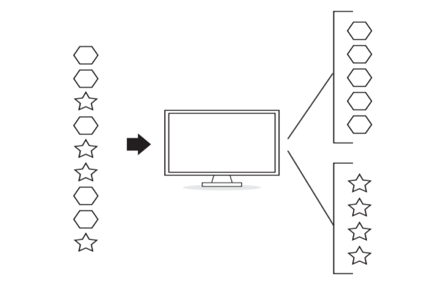
\includegraphics[width=7.5cm]{figuras/clustering}
\caption{Tarefa de clusterização. Não há uma distinção entre etapas de treinamento e de previsão. O algoritmo agrupa os dados a ele fornecidos e dá a resposta diretamente.\footnote{Extraído de \citep{allen}}}
\label{fig:clustering}
\end{figure}

Outra técnica do aprendizado não-supervisionado é a \defi{detecção de anomalias}, cujo objetivo é ter uma descrição de como os dados considerados ``normais'' se parecem, e usa-se esse agrupamento para detectar se novos dados estariam ``fora'' desse padrão. Um exemplo é a detecção de fraudes.

Por último, pode-se citar a técnica de \defi{estimação de densidades}, que tem como objetivo a estimação da função densidade de probabilidade de um conjunto de dados gerados por algum processo aleatório.

Existe também o \defi{aprendizado semi-supervisionado} em que combinam-se vantagens de ambos os tipos anteriores. Um modelo utiliza dados sem rótulos para descobrir uma estrutura geral dos dados, enquanto usa alguns poucos rótulos conhecidos para ajudar na organização inicial dessa estrutura, o que auxilia no agrupamento, que é um exemplo de problema não-supervisionado.

Essa técnica é também conhecida por \emph{aprendizagem fraca}, e conforme aponta Allen \citep{allen} possui a vantagem de precisar de menor quantidade de dados rotulados para que se alcance um bom resultado em termos de qualidade do modelo, já que aprende parte do padrão dos dados a partir dos dados sem rótulos. Na prática, pode-se e deve-se testar várias abordagens, e a escolha é mais baseada nos resultados do que na teoria de que uma técnica ou outra irá se sair melhor para um problema específico.

Uma técnica já bem diferente das anteriores, é a \defi{aprendizado por reforço} (\eng{reinforcement learning}). Allen \citep{allen} nos explica o conceito principal dessa abordagem, que consiste na existência de um ``agente'' que interage executando ações num ``ambiente'', que dá um retorno (\eng{feedback}) a esse agente, usualmente na forma de uma ``recompensa''. Tal recompensa pode ser entendida especificamente como um contador. 

O objetivo do agente é maximizar esse contador. Nenhuma informação é dita ao agente sobre como ele aumenta esse contador, ou porquê ele conseguiu aumentar, ele irá definir suas ações de acordo com as respostas dadas pelo ambiente. Assim, tudo que ele sabe é se houve a recompensa ou não, e irá preferir as ações que fizeram o contador aumentar e preterir aquelas que fizeram ele diminuir, sem nunca existir rótulos ou respostas conhecidas.

\subsection{O problema do sobreajuste dos modelos}

O sobreajuste (\eng{overfitting}) é o primeiro desafio que deve ser enfrentado quando realizados uma tarefa de aprendizado de máquina. Um modelo de aprendizado de máquina só é considerado válido ou útil, quando está treinado de forma que sofre de pouquíssimo, ou, idealmente, nenhum sobreajuste.

O sobreajuste ocorre quando um modelo foi treinado exageradamente para o conjunto de dados conhecidos, ou seja, o conjunto utilizado para o treino. De forma que, ao se deparar com dados novos, desconhecidos, perde a capacidade de saber o que fazer, ou seja, erra muito nas previsões ao mesmo tempo que está com um desempenho quase perfeito no conjunto de treino. 

Isto pode ocorrer em qualquer tarefa de aprendizado supervisionado, tanto nas de classificação, quanto nas de regressão. Utilizando o exemplo dado por Allen \citep{allen}, imaginemos um modelo de classificação de fotos de animais. Um modelo $100\%$ sobreajustado irá \emph{decorar} as cores de cada um dos pixels dessa imagem, de forma que todos eles serão necessários para ele identificar se tal foto é um gato, ou um cachorro, etc.

Mudando apenas a cor ou a posição de um dos pixels de uma das imagens, e supondo que essa imagem modificada não fazia parte do conjunto de imagens do treinamento, o modelo não será capaz de fornecer uma resposta válida ou confiável. A Figura \ref{fig:over_class} ilustra esse exemplo.

\begin{figure}[htb]
\centering
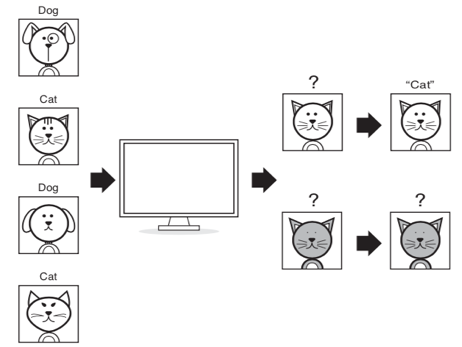
\includegraphics[width=7.5cm]{figuras/over_class}
\caption{Sobreajuste num modelo de classificação.\footnote{Extraído de \citep{allen}}}
\label{fig:over_class}
\end{figure}

Ou seja, o modelo fica perfeito para os dados de treino, mas fica totalmente cego para os dados do mundo real, desconhecidos. O problema do sobreajuste também está presente nos modelos de regressão. Consideremos o exemplo dado por Allen \citep{allen}.

Considere um gráfico que relaciona a metragem ao quadrado de terrenos, no eixo $X$ com o valor pago por eventuais compradores, no eixo $Y$. Um problema típico de regressão é o da determinação do valor da compra ou venda de um terreno em termos de sua metragem. 

O modelo mais simples seria o de uma regressão linear, explicado em detalhes na próxima seção, em que basicamente, traçamos uma reta do tipo $y = bx + a$, cujo valor $y$ irá servir de valor esperado para nosso modelo, para qualquer outro $x$. Uma ilustração desse modelo hipotético está na Figura \ref{fig:over_reg_1}.

\begin{figure}[htb]
\centering
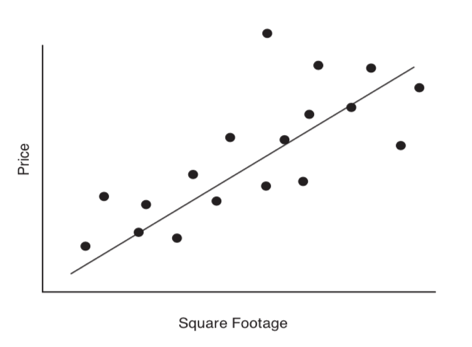
\includegraphics[width=7.5cm]{figuras/over_reg_1}
\caption{Modelo de regressão, ajuste linear.\footnote{Extraído de \citep{allen}}}
\label{fig:over_reg_1}
\end{figure}

Podemos não ficar satisfeitos com esse ajuste linear, já que praticamente nenhum ponto está contido perfeitamente na reta ajustada. E assim, supomos um novo modelo, dessa vez de um polinômio de grau $m < N$ ($N$ é o número de pontos), isto é, um modelo do tipo $y = a_mx^m + a_{m-1}x^{m-1} + \ldots + a_1x + a_0$. A diferença é que antes tínhamos $2$ parâmetros, e agora temos $m{+}1$ parâmetros para estimar.\footnote{É importante mencionar que, em outros contextos, o número de parâmetros livres de um modelo é conhecido como o número de \emph{graus de liberdade} desse modelo.} Um ajuste possível, é ilustrado na Figura \ref{fig:over_reg_2}.

\begin{figure}[htb]
\centering
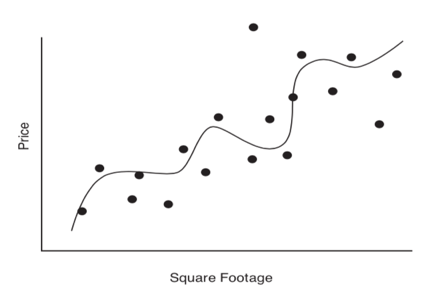
\includegraphics[width=7.5cm]{figuras/over_reg_2}
\caption{Modelo de regressão, polinômio de grau $m$.\footnote{Extraído de \citep{allen}}}
\label{fig:over_reg_2}
\end{figure}

Aparentemente, esse modelo é melhor do que o anterior, pois a função está melhor ajustada aos dados conhecidos. Poderíamos pensar que quanto mais parâmetros, isto é, quanto maior o grau do polinômio a ser ajustado, mais adequado o modelo estará aos dados. 

Isso pode chegar até o extremo em que, possuindo $N{+}1$ dados, ajustamos um polinômio de grau $N$ aos dados. Tal ajuste está ilustrado na Figura \ref{fig:over_reg_3}.

\begin{figure}[htb]
\centering
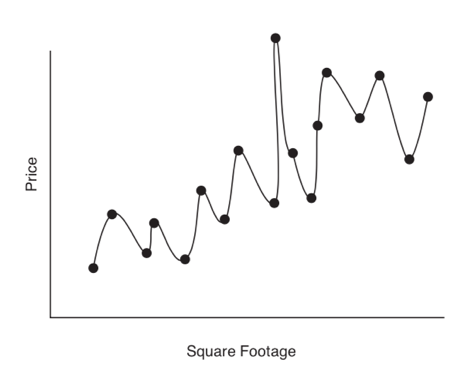
\includegraphics[width=7.5cm]{figuras/over_reg_3}
\caption{Modelo de regressão, polinômio de grau $N$.\footnote{Extraído de \citep{allen}}}
\label{fig:over_reg_3}
\end{figure}

Com isso, teremos o caso extremo de um modelo de regressão totalmente sobreajustado. Ele está perfeitamente ajustado aos dados conhecidos, mas retornará resultados espúrios para qualquer outro $x$ que não pertença a esse conjunto, perdendo a capacidade de \emph{generalização}, conforme explicado por Allen \citep{allen}.

O objetivo dessa discussão é apontar que devemos ser parcimoniosos na escolha do nosso modelo, tentando buscar aquele com o menor número possível de parâmetros a serem ajustados, de modo a buscar ao mesmo tempo um bom desempenho no conjunto de treinamento (mas não perfeito), e também uma capacidade igualmente boa de generalização para os dados cuja resposta é desconhecida.

Outras técnicas também podem ser utilizadas quando estamos lidando com o sobreajuste de modelos. Daniil Korbut \citep{korbut} citam as técnicas de regularização, que são úteis para se evitar o sobreajuste nos modelos de aprendizado.

\section{Algoritmos básicos de aprendizagem}

Conhecendo os tipos mais comuns de aprendizagem, o próximo passo nesse caminho da ciência de dados é conhecer os diferentes algoritmos de aprendizagem, alguns sendo mais usados em tarefas supervisionadas, outros em tarefas não-supervisionadas e alguns podendo ser utilizados em ambos os tipos de tarefas.

É importante também conhecer para quais tarefas eles foram concebidos, pois essa etapa é muito importante, dentro do contexto humano da ciência de dados, para se adquirir intuição e auxiliar na escolha do algoritmo ou dos algoritmos mais úteis que possam modelar algum novo problema.

\subsection{Regressão Linear}

Regressão linear é um dos problemas pioneiros e mais simples de aprendizagem de máquina supervisionada. Desenvolvido em \emph{estatística}, este problema possui soluções com fórmulas bem definidas como o método dos mínimos quadrados.

O uso de técnicas computacionais iterativas é muito bem-vinda, se estamos lidando com volumes de dados muito grandes, e que exigem operações sobre matrizes, como multiplicação, inversão, diagonalização, etc.

Formalmente, supomos um modelo de regressão linear múltipla, associando um conjunto de variáveis independentes $X_1, X_2, \ldots, X_p$, a uma variável dependente $Y$, que representa a resposta esperada. Juntos eles representam os dados, e dessa forma escrevemos o seguinte modelo.

\begin{equation}\label{algo:1}
Y = \beta_0 + \beta_1 X_1 + \ldots + \beta_p X_p + \epsilon \; ,
\end{equation}
onde $\epsilon$ é um erro aleatório, para o qual assume-se uma distribuição normal de média~$0$.

Temos portanto $p{+}1$ parâmetros a serem ajustados em nosso modelo. Uma solução conhecida para o caso univariado, retirada de Magalhães e Lima \citep{antonio} (páginas $332{-}336$), e que pode ser generalizada, é dada pelo método dos mínimos quadrados. 

Se possuímos $n$ observações disponíveis, tanto das variáveis independentes $X_i$ quanto das variáveis dependentes $Y_i$, e denotando da seguinte maneira:

\[
Y = \left[ \begin{array}{c} Y_1 \\ Y_2 \\ \vdots \\ Y_n \end{array} \right], \;
X = \left[ \begin{array}{cccc} 1 & x_{11} & \ldots & x_{1p} \\ 1 & x_{21} & \ldots & x_{2p} \\ \vdots & \vdots & \ddots & \vdots \\ 1 & x_{n1} & \ldots & x_{np} \end{array} \right], \;
\beta = \left[ \begin{array}{c} \beta_0 \\ \beta_1 \\ \vdots \\ \beta_p \end{array} \right], \;
\epsilon = \left[ \begin{array}{c} \epsilon_1 \\ \epsilon_2 \\ \vdots \\ \epsilon_n \end{array} \right]
\]

Usando essa notação, podemos reescrever a equação (\ref{algo:1}), para $n$ observações:

\begin{equation}\label{algo:2}
Y = X \beta + \epsilon \; .
\end{equation}

Esse problema possui uma solução algébrica dada pelo método dos mínimos quadrados, que nos fornece a estimativa $\hat{\beta}$ do vetor $\beta$, dada por:
\begin{equation}\label{algo:3}
\hat{\beta} = (X'X)^{-1}X'Y \; ,
\end{equation}
onde $X'$ é a matriz $X$ transposta, e que assume uma definição baseada na minimização da função de erro quadrático, feita de forma algébrica. 

As técnicas de aprendizado de máquina entram em jogo se queremos utilizar uma outra função de erro, ou se queremos uma outra abordagem para a minimização da função de erro escolhida, como por exemplo o método do gradiente descendente, explicado em detalhes no Apêndice \ref{ap:gradiente}.

A utilização do gradiente descendente ou de outro método de otimização qualquer é motivada pela maior eficiência computacional desses métodos em comparação com a inversão de matrizes de ordem $p{\times}p$ necessária no cálculo direto de \eqref{algo:3}. A justificativa é facilmente verificada em problemas do mundo real, onde, na maioria dos casos, $p$ é um número grande.

As técnicas de regularização, já citadas anteriormente, tem um papel importante no ajuste de modelos de regressão. A ideia é adicionar parâmetros sem importância prática às somas dos quadrados na função de erro quadrático, com o objetivo de minimizar os valores dos parâmetros de interesse. Explicações mais detalhadas podem ser encontradas em Géron \citep{hands} (páginas $196{-}205$).

É possível utilizar a abordagem puramente estatística, lidando diretamente com as Equações \eqref{algo:2} e \eqref{algo:3}; entretanto, a vantagem de se utilizar técnicas computacionais eficientes permanece imprescindível quando o número de parâmetros ($p$) é grande.

\subsection{Regressão Logística}

Suponhamos agora que queremos prever a probabilidade de que algo ocorra. Por exemplo, queremos decidir, a partir de uma base de dados de características de clientes conhecidos e de suas compras, se um novo cliente, dadas apenas suas características, irá comprar um certo produto.

Se assumirmos que estamos usando características independentes, nada nos impediria de aplicarmos a modelagem da regressão linear vista anteriormente. O resultado seria uma função que dada a lista de características de um cliente novo, retornaria um número real. Esse número porém, sofreria de problemas de interpretação.

Poderíamos supor que se o número retornado fosse grande, então haveria alta probabilidade do cliente comprar, ou se o número retornado fosse muito pequeno, ou até mesmo negativo, que ele teria baixa probabilidade de comprar o produto. Mas essa linha de decisão seria ruim, pois, o que nos garantiria que essa interpretação representaria a realidade?

Uma alternativa é modelarmos em termos de probabilidades reais, ou seja, um modelo cuja resposta fosse um número entre $0$ e $1$, de forma que a interpretação probabilística fosse muito mais natural. Esta é a motivação do modelo de regressão logística.

Por causa da natureza da previsão, que irá retornar basicamente, sim ou não, este pode ser considerado um algoritmo de classificação, apesar do nome e do funcionamento interno	caracterizarem-no como uma regressão. Além disso, é um algoritmo supervisionado, já que nosso modelo é construído utilizando dados já observados de compras de clientes.

Para o caso em que a variável dependente ($Y_i$) assumir apenas dois possíveis estados ($1$ ou $0$) o modelo é dado, para cada observação ($X_i, Y_i$), por:

\begin{equation}\label{log:f}
P(Y_i = 1) = \frac{1}{1 + e^{-f(X_i)}}
\end{equation}
em que $f(X_i)$ é, como na expressão da regressão linear, dado por:

\[ f(X_i) =  X_i \beta + \epsilon_i \; . \]

O que queremos fazer é maximizar a probabilidade de que os dados com valores conhecidos assumam os valores esperados de $Y_i$. Esta probabilidade é definida, em Grus \citep{data}, por:
\begin{equation}\label{log:veros}
P(Y_i{=}y_i | X_i{=}x_i, \beta) = f(x_i \beta)^{y_i} (1 - f(x_i \beta))^{1-y_i}
\end{equation}
em que, $y_i = 1$ ou $y_i = 0$, para toda observação indexada por $i$.

Nesse modelo o parâmetro a ser estimado é $\beta$, que será o mesmo para todas as observações. Fazendo o produto de todas as observações, onde para cada uma usamos a mesma expressão (\ref{log:veros}), teremos a \emph{verossimilhança} da amostra. Assim, desejamos um algoritmo que irá maximizar a verossimilhança, ou ainda a log-verossimilhança de nossa amostra, e irá retornar a estimativa $\hat{\beta}$.

Novamente, no contexto de aprendizado de máquina, o mais eficiente será utilizar algum algoritmo de gradiente descendente estocástico, para realizar esse trabalho, motivo pelo qual é tratado como um algoritmo de aprendizagem, em oposição ao procedimento do cálculo direto de $\hat{\beta}$.

A seguir, com o $\hat{\beta}$ em mãos, poderemos classificar novos clientes, aplicando suas características de volta na expressão (\ref{log:f}), com o $\hat{\beta}$ ajustado. A resposta será um número no intervalo $[0, 1]$, para o qual poderemos definir um \emph{corte}, sendo o mais simples definir que, se esse número for maior ou igual a $0.5$ diremos que o cliente irá comprar, caso contrário, não irá comprar.

Alternativamente, podemos ter como resposta direta o número calculado, para então gerarmos estratégias distintas para clientes com \emph{alta}, \emph{média} ou \emph{baixa} probabilidade de compra de certo produto, por exemplo.

\subsection{Árvores de decisão}

Uma \defi{árvore de decisão} é um outro exemplo de algoritmo supervisionado usado principalmente para classificação, mas que também pode ser usada para regressão. É definida por Grus \citep{data} como sendo uma estrutura que representa um número de possíveis caminhos de decisão e um resultado para cada caminho.

Apesar dessa vaga definição, um exemplo muito útil é o da classificação das famílias pertencentes ao reino vegetal, na Figura \ref{fig:plantas}, sem nos preocuparmos com os detalhes biológicos.

\begin{figure}[htb]
\centering
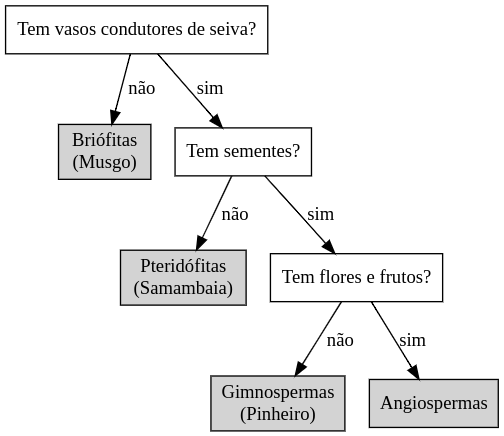
\includegraphics[width=8cm]{figuras/plantas}
\caption{Árvore de decisão classificando famílias de plantas.}
\label{fig:plantas}
\end{figure}

Pode-se notar a natureza didática das árvores de decisão, pois elas são de fato intuitivas. Dada uma planta, fizemos perguntas simples e diretas sobre suas características, que estão representadas pelos quadros de fundo branco de onde saem flechinhas indicando as respostas negativas e positivas; estes quadros são os \defi{nós de decisão}.

Seguir as flechas, ou seja, as decisões de cada pergunta ou característica, nos permitirá classificar uma planta em alguma das famílias representadas pelos quadros de fundo cinza, de onde não saem mais flechinhas. Estes são os \defi{nós-folhas}, que são as respostas dadas por essa árvore de classificação.

Isto nos leva ao funcionamento do algoritmo de uma árvore de decisão. Segundo Grus \citep{data}, para construir uma árvore de decisão, precisamos decidir quais perguntas fazer e em qual ordem. Cada pergunta irá separar as possibilidades restantes de acordo com as respostas. 

Outro aspecto importante é decidir os \emph{cortes} de cada pergunta, ou seja, se estamos lidando com valores contínuos (por exemplo, o tamanho do caule), então será preciso definir, como no caso da regressão logística, um valor que será o limiar entre uma resposta negativa e positiva para essa pergunta (por exemplo, \emph{o caule é grande?}).

De acordo com Grus \citep{data}, seria útil escolher perguntas cujas respostas darão muita informação sobre o que a árvore deverá prever. Esta informação pode ser mensurada com o conceito de \defi{entropia}, que neste contexto, representa a incerteza associada aos dados.

Seja um conjunto de dados $S$, para os quais podemos rotular uma dentre $n$ classes, $C_1, \ldots, C_n$. Se todos os dados de $S$ possuírem a mesma classe, a entropia $H$ de $S$ será zero. Se os pontos estiverem igualmente espalhados entre as classes, então a entropia será a máxima possível.

De modo geral, se $p_i$ é a proporção de dados que pertencem à classe $C_i$, então a entropia de $S$ será:
\begin{equation}\label{eq:entropia_1}
H(S) = -p_1 \log_2 p_1 - \ldots - p_n \log_2 p_n \; ,
\end{equation}
sendo que Grus \citep{data} utiliza a convenção: $0 \log 0 = 0$.

Se analisarmos rapidamente cada termo, como uma função $f(p) = {-p} \log p$, estendida com a convenção acima, vemos que é uma função que se aproxima de $0$ quando $p$ se aproxima de $0$ ou de $1$, e se afasta de $0$, caso contrário, isto é, tem uma concavidade negativa, cruzando o eixo nos pontos $p=0$ ou $p=1$.

Assim, a entropia de $S$ será maior quando os dados estiverem mais espalhados, o que significa que há maior incerteza na base, enquanto que será menor quando os dados estiverem mais concentrados em poucas classes, o que indicaria menor incerteza, o que configura o comportamento que gostaríamos de obter.

Sabendo calcular a entropia do conjunto total $S$ que representa uma \emph{árvore}, o próximo passo é calcular a entropia de \emph{ramos} da árvore, que serão obtidas a partir de perguntas que irão separar o conjunto $S$ em dois ou mais subconjuntos.

Se estamos lidando com características categóricas, cada valor assumido por essa característica é uma das respostas possíveis, gerando um ramo para cada, ou seja, uma seta de decisão. Se uma característica é numérica e contínua, daí há uma liberdade na escolha da pergunta, podendo ser usada por exemplo a média ou a mediana para separar os dados abaixo ou acima desse corte.

Generalizando a mesma definição anterior, se dividirmos os dados de $S$ em subconjuntos $S_1, \ldots, S_m$, para uma característica com $m$ valores distintos possíveis, cada um contendo proporções $q_1, \ldots, q_m$ respectivamente, então a entropia da árvore será a soma ponderada das entropias de cada ramo:

\begin{equation}\label{eq:entropia_2}
H(S) = q_1 H(S_1) + \ldots + q_m H(S_m) \; ,
\end{equation}
em que cada termo $H(S_i)$ é obtido normalmente por (\ref{eq:entropia_1}).

A partir dessa definição, já podemos construir um primeiro algoritmo de árvore de decisão. De acordo com Grus \citep{data}, um algoritmo \emph{ganancioso}, pode ser construído como se segue. Dadas as características presentes em $S$, ou seja, as variáveis explicativas, calculamos para cada uma o valor $H$ dado por (\ref{eq:entropia_2}).

Escolhemos como nosso primeiro nó de decisão, a característica que nos der o menor valor de entropia $H$. Com isso, sabemos que essa característica é a que melhor separa as classes, que serão os nós folhas (as respostas), ao menos nesse momento.

Assim obtemos $2$ ramos, e em cada um deles podemos repetir esse mesmo procedimento. Se fizermos isso para todas as características, então cada ramo de nossa árvore poderá eventualmente conter apenas uma das classes possíveis, o que seria perfeito para o conjunto de treino, mas seria péssimo para dados novos, pois nossa árvore estaria completamente \emph{sobreajustada}.

É por isso que para um modelo de árvore de decisão, existem comumente $2$ \defi{hiperparâmetros}\footnote{Parâmetros inerentes ao modelo e não aos dados, e que devem ser escolhidos durante a parte prática do treinamento do algoritmo.} muito importantes segundo Korbut \citep{korbut}, que são o número máximo de nós de decisão, ou seja, o número de perguntas e o número mínimo de nós folhas, ou seja, de classes por ramo.

Ajustando esses parâmetros, podemos garantir que uma árvore não-perfeita mas boa o suficiente para o conjunto de treino seja igualmente boa para o conjunto de teste, e dessa forma, para dados desconhecidos, para que ela seja útil para a tarefa de classificação proposta.

Por fim, vale citar a ressalva de Korbut \citep{korbut} de que um modelo utilizando apenas uma árvore é raramente usado. Mas combinando várias árvores criamos os algoritmos chamados de \emph{florestas aleatórias} (\eng{random forests}), que estão dentre os mais versáteis e utilizados para tarefas de classificação.

\subsection{$K$-médias}

O $k$-médias (\eng{$k$-means}) é o ponto central de todas as tarefas de aprendizado não-supervisionadas conhecidas como \defi{agrupamento}. A ideia é agrupar os dados de acordo com um conceito de \emph{distância} e com a suposição de que \emph{proximidade} implica \emph{similaridade} no espaço em que calculamos essas distâncias.

O procedimento geral é agrupar os dados em $k$ agrupamentos, em que, cada grupo terá uma \emph{média} que irá caracterizar esse grupo, daí o nome do algoritmo. Segundo Korbut \citep{korbut}, podemos partir de $k$ pontos escolhidos aleatoriamente e nomeá-los como os centros (ou médias) de cada grupo.

A seguir, calculamos as distâncias de cada ponto aos centros, e incluímos em cada grupo aqueles pontos que estão mais próximos de algum dos centros. Isto é, dado um ponto, incluímos ele no grupo que possui o centro que está mais próximo dele.

Então, o centro real de cada grupo é calculado (a média, por exemplo), e o processo acima se repete. Esse ciclo é repetido, idealmente, até que haja convergência, ou seja, calcular a média dos grupos não altera a pertinência de mais nenhum ponto dentre os $k$ grupos.

O grande desafio é, justamente, a escolha de $k$, que é a princípio desconhecido. Khyati Mahendru \citep{means} explica dois métodos que podem ser úteis na escolha do melhor $k$: o \emph{método do cotovelo} (\eng{Elbow method}), e o \emph{método da silhueta} (\eng{Silhouette method}). Ela explica que ambos os métodos são ferramentas complementares, isto é, não alternativas entre si, sendo utilizadas em conjunto para uma escolha mais confiável de $k$.

Além disso, para $k$ pontos iniciais escolhidos, pode haver uma convergência local dos agrupamentos, e não global, análogo ao problema de maximização/minimização global de funções.

\section{As redes neurais e o \emph{perceptron}}

De acordo com Géron \citep{hands}, as primeiras redes neurais foram introduzidas em 1943 pelo neurofisiologista Warren McCulloch e o matemático Walter Pits através de um modelagem computacional do funcionamento conjunto de neurônios no cérebro de animais, enquanto realizam complexos cálculos lógicos. Esta foi a primeira \defi{arquitetura} de uma rede neural artificial.

Esse começo promissor levou as pessoas a acreditarem que logo haveriam máquinas realmente inteligentes, o que ficou registrado na cultura da época, principalmente em séries televisivas de ficção científica como \eng{Star Trek} e outras, mas conforme aponta Géron \citep{hands}, essa promessa logo se mostrou inalcançável, ao menos era o que parecia ao final dos anos 60. 

A partir dos anos 80, surgiram novas arquiteturas e melhores técnicas de aprendizagem, embora sua evolução fosse lenta devido ao poder computacional limitado da época. Atualmente, no entanto, isto mudou: há poder computacional em casa e na nuvem, há a internet e fóruns de compartilhamento de códigos e conhecimentos em programação e ciência de dados, em resumo o mundo atual está consolidado numa era digital. 

Por essa razão Géron \citep{hands} nos diz que estamos numa nova onda de entusiasmo sobre as redes neurais, sendo que esse entusiasmo leva o nome de \defi{Deep Learning}, ou aprendizado profundo, e o uso desse adjetivo ajuda a descrever as redes neurais, constituídas de milhares de neurônios, que são utilizadas em várias aplicações de nosso dia-a-dia na internet.

Podemos citar a classificação de bilhões de imagens realizadas pelo \emph{Google}\footnote{\url{https://developers.google.com/earth-engine}}, reconhecimento de fala realizado pela \emph{Siri} da \emph{Apple}\footnote{\url{https://machinelearning.apple.com/research/siri-voices}}, o sistema de recomendações de vídeos em plataformas de \emph{streaming}, como \emph{Youtube} e \emph{Netflix}\footnote{\url{https://towardsdatascience.com/deep-dive-into-netflixs-recommender-system-341806ae3b48}}, e até mesmo os jogadores artificiais de xadrez\footnote{\url{https://www.nytimes.com/2018/12/26/science/chess-artificial-intelligence.html}}. As redes neurais estão vivas em nosso mundo. Mas como funcionam na prática, por detrás dessa aparência de ficção científica?

Uma definição para uma rede neural dada por Rosangela Ballini \citep{doutorado} é a de um sistema de processamento paralelo e distribuído construído em um formato e com funcionalidade que se parece com o arranjo de um sistema nervoso biológico, sendo compostos por elementos computacionais chamados neurônios, que são organizados e interligados em padrões semelhantes aos neurônios biológicos.

Na Figura~\ref{fig:neuron} está uma representação de um neurônio biológico. Ele recebe impulsos elétricos de entrada através dos dendritos, que são transmitidos ou não através do núcleo, caso sejam ativados por ele, para os terminais de saída dos axônios. Os neurônios se comunicam através de sinapses, que são ligações entre os dendritos de um e os axônios de outro que realizam a transmissão dos sinais. 

\begin{figure}[htb]
\centering
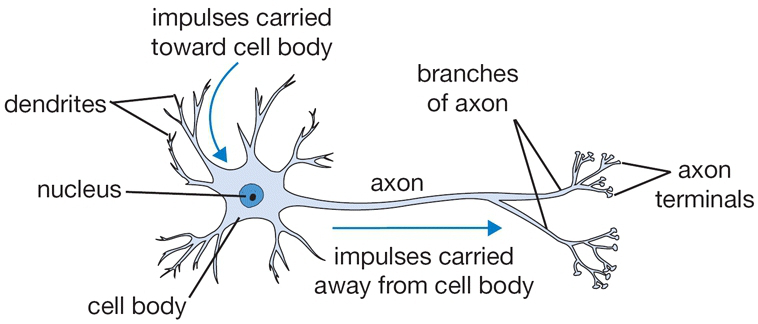
\includegraphics[width=8cm]{figuras/neuron}
\caption{Representação de um neurônio biológico.\footnote{Extraído de \url{https://cs231n.github.io/neural-networks-1/}}}
\label{fig:neuron}
\end{figure}

Dá-se o nome de \eng{perceptron} de camada única (\eng{single-layer perceptron}) ou simplesmente \eng{perceptron} a uma das mais simples arquiteturas de rede neural, criada em 1957 por Frank Rosenblatt \citep{frank}. Uma ilustração conceitual dela está na Figura~\ref{fig:perceptron}. Existem atualmente diversas outras arquiteturas de redes neurais, mas a extensão mais imediata que podemos citar de um \eng{perceptron} constituído de uma camada de neurônios são as redes \eng{perceptron} multi-camadas (\eng{multi-layer perceptron}). 

Os neurônios são representados por círculos, dentro deles há um valor numérico que intuitivamente podemos atribuir ao nível ou grau de ativação do neurônio, mesmo que no caso biológico se restrinja aos valores $0$ e $1$, ou seja, ativado ou não. Cada coluna de neurônios representa uma camada, nesse caso, da esquerda para a direita temos a camada de entrada, a camada oculta e a camada de saída. As linhas representam as ligações entre os neurônios, sendo que cada neurônio de uma camada está ligado a todos da camada anterior.

\begin{figure}[htb]
\centering
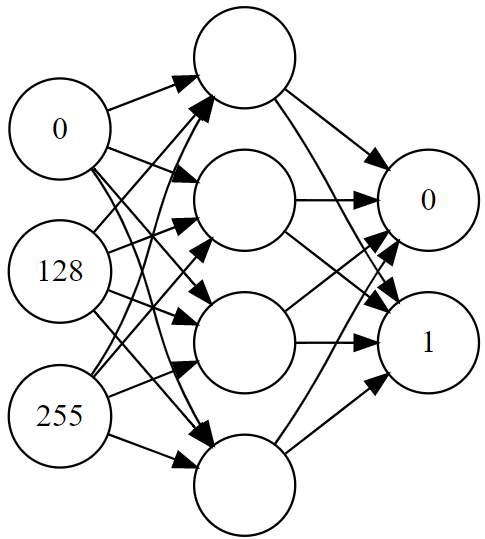
\includegraphics[width=5cm]{figuras/perceptron}
\caption{Rede neural simples, o \eng{perceptron} de camada única.}
\label{fig:perceptron}
\end{figure}

O \eng{perceptron} de camada única consiste de uma camada de neurônios de entrada, uma camada oculta de neurônios usados na otimização, e uma camada de saída, que irá conter os dados previstos, ou ainda as probabilidades do dado pertencer a alguma das classes na qual a rede poderá classificá-lo. E é o fato de haver uma camada oculta nesta rede que a define como sendo de ``camada única''. Caso houvessem mais do que uma camada oculta, ela seria do tipo ``multi-camadas'' mencionado acima.

De modo a entendermos as bases matemáticas do algoritmo, podemos começar com uma rede ainda mais básica, a partir de um \eng{perceptron} que seja constituído de apenas $1$ neurônio na única camada oculta. Esta rede super simplificada, que está na Figura~\ref{fig:neuronio}, pode ser útil para para o entendimento uma vez que neste caso será possível acompanhar graficamente o resultado da execução do algoritmo.

\begin{figure}[htb]
\centering
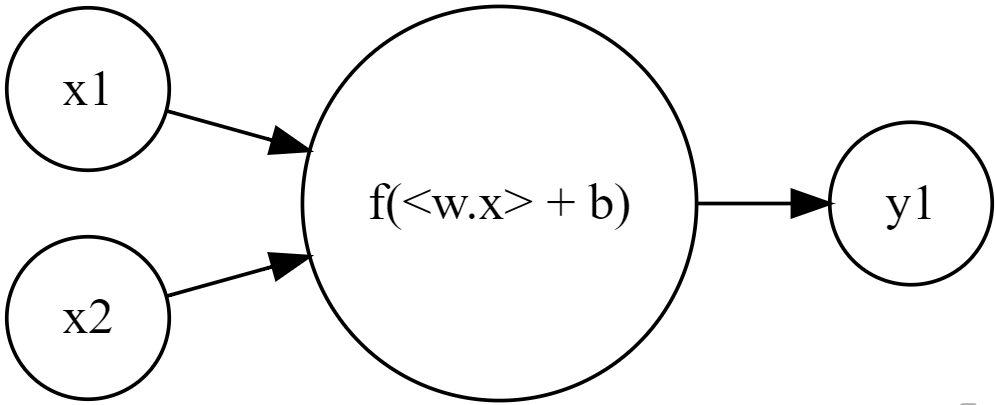
\includegraphics[width=8cm]{figuras/neuronio}
\caption{Rede neural mais simples, apenas um neurônio oculto.}
\label{fig:neuronio}
\end{figure}

Esta rede possui $2$ neurônios na camada de entrada, que são os números reais $x_1$ e $x_2$, $1$ neurônio na camada oculta, no qual está a sua função de ativação $f(x_1w_1 + x_2w_2 + b)$, e $1$ neurônio na camada de saída, que neste caso é um número real $y_1$. Pode-se notar a semelhança dessa rede neural artificial com a sua inspiração biológica com a ajuda da Figura~\ref{fig:neuron_model}. 

\begin{figure}[htb]
\centering
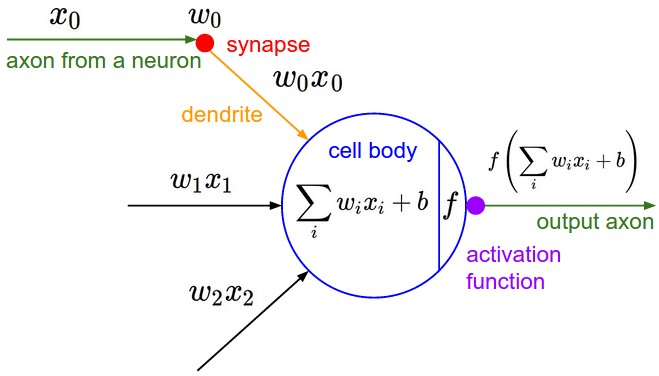
\includegraphics[width=8cm]{figuras/neuron_model}
\caption{Representação de um neurônio artificial.\footnote{Extraído de \url{https://cs231n.github.io/neural-networks-1/}}}
\label{fig:neuron_model}
\end{figure}

Temos os sinais de entrada ($x_1$ e $x_2$) representando os sinais recebidos dos axônios de outros neurônios. Eles entram pela camada de entrada da rede, ou dendritos do neurônio. A camada oculta processa as entradas com os pesos, definindo o formato final do sinal através de sua função de ativação, que aqui pode ser uma função real qualquer, mas com funcionalidade similar ao do núcleo do neurônio que ativa/transmite ou não o sinal recebido por ele. Por fim o sinal é enviado à camada de saída, ou aos axônios do neurônio, concluindo o processamento.

A partir desta analogia podemos compreender o funcionamento básico da rede neural \eng{perceptron}. Ela recebe uma lista de valores como entrada, que podemos representar por um vetor real $x$. O neurônio oculto representa uma transformação linear neste vetor, que podemos escrever como o produto escalar por um outro vetor real, o vetor de \defi{pesos} $w$, ou seja, $\langle w x \rangle$, que é o produto escalar usual dos números reais. A seguir, somamos um outro número real $b$ que é chamado de \defi{viés}, que possui o mesmo papel que a constante de interceptação da reta com o eixo vertical de um ajuste linear.

Por fim, é aplicada uma função de ativação não-linear sobre esta transformação, o que configura a saída deste neurônio: $f(\langle w x \rangle + b)$, que é transmitida ao neurônio de saída, que pode aplicar uma transformação semelhante ou outra qualquer, dependendo da função de ativação utilizada em cada camada da rede. Mostramos uma rede bem simples, mas na prática podem haver muito mais camadas ocultas, e cada uma delas, assim como a camada de saída, muitos neurônios cada.

Este processo de entrada, processamento e saída da rede é chamado de \defi{feedforward}, e consiste no nível mais fundamental do \eng{perceptron}. A partir daí, a forma como a rede será treinada, é o que define se ela será utilizada para um aprendizado supervisionado ou não-supervisionado.

Uma vez que estamos lidando com o aprendizado supervisionado, deve ser utilizado um algoritmo de treinamento que forneça à rede pares conhecidos de vetores de entradas e saídas esperadas, e um \defi{critério de avaliação} de quão boa é a performance da rede para aproximar as suas saídas às saídas esperadas.

Este critério é uma função que fornece uma medida da distância entre as saídas obtidas pela rede e as saídas esperadas, que é genericamente chamada de função de custo (\eng{cost function}). Se denotarmos por $y$ uma saída conhecida, e por $a^{(L)}$ uma saída obtida pela última camada, exemplos comumente usados são as normas usuais como a distância euclidiana $(a^{(L)^2} + y^2)^{1/2}$, a função de erro absoluto $|a^{(L)} - y|$, e a função de erro quadrático $(a^{(L)} - y)^2$, que é a usada no algoritmo descrito por Kopec \citep{classic} e que será usada neste trabalho.

Um dos algoritmos de treinamento que minimizam uma função de custo é o gradiente descendente (\eng{gradient descent}), que segundo Géron \citep{hands} é um algoritmo que serve para encontrar soluções ótimas para uma grande variedade de problemas de otimização. Detalhes de seu funcionamento podem ser vistos no Apêndice \ref{ap:gradiente}.

\section{Arquiteturas de redes neurais}

Existem dezenas de arquiteturas de redes neurais artificiais, como pode ser observado examinando-se a quantidade de arquiteturas listadas no website \emph{The neural network zoo}\footnote{\url{https://www.asimovinstitute.org/neural-network-zoo/}}, o que demonstra que esse assunto é levado muito a sério. A representação gráfica ali criada é útil para o entendimento das características das diversas arquiteturas, graças aos padrões de cores e de formas geométricas utilizadas.

A primeira estrutura é o \eng{perceptron} simples, de apenas um neurônio, que processa $n$ entradas através de uma transformação linear seguida de uma função de ativação. É exibido no canto superior esquerdo da Figura \ref{fig:estrutura_p}.

\begin{figure}[htb]
\centering
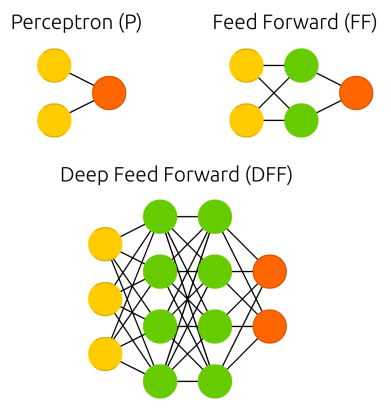
\includegraphics[width=7cm]{figuras/estrutura_p}
\caption{As redes neurais recorrentes: \eng{perceptron}, \eng{feedforward} e \eng{deep feedforward}.\footnote{Extraído de \url{https://www.asimovinstitute.org/neural-network-zoo/}}}
\label{fig:estrutura_p}
\end{figure}

No canto superior direito está a versão \eng{feedforward}, possuindo uma camada oculta representada pelos círculos verdes, e embaixo está a versão \eng{deep feedforward}, que possui múltiplas camadas ocultas, e número variado de neurônios em todas as camadas, e é de fato a versão que foi implementada nesse trabalho.

As características em comum das arquiteturas derivadas da rede \eng{perceptron}, chamadas de \defi{redes neurais sequenciais}, são: a conexão que existe entre cada neurônio de uma camada com todos os neurônios da camada anterior, e a forma que a informação é transmitida da rede, num sentido único, da camada de entrada, os círculos amarelos, para a camada de saída, os círculos vermelhos.

A próxima arquitetura em destaque define o que são as \defi{redes neurais recorrentes}, ilustrada na Figura \ref{fig:estrutura_r}. Nesse tipo de rede a informação pode ir para frente e para trás, além disso pode passar pelo mesmo neurônio oculto mais de uma vez, o que determina o nome recorrente. Esses neurônios são representados pela cor azul na Figura.

\begin{figure}[htb]
\centering
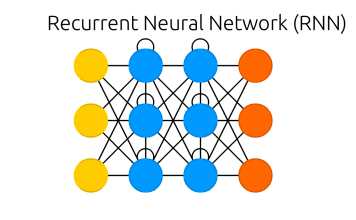
\includegraphics[width=7cm]{figuras/estrutura_r}
\caption{As redes neurais recorrentes.\footnote{Extraído de \url{https://www.asimovinstitute.org/neural-network-zoo/}}}
\label{fig:estrutura_r}
\end{figure}

Esse tipo de rede, segundo Kopec \citep{classic} é a mais usada em problemas em que os dados utilizados possuem uma dependência da ordem em que são obtidos e possuem entradas contínuas. Por exemplo, os dados de uma série temporal de dados, em que a previsão de um dado, que representaria o futuro, depende da ordem em que estão os dados já conhecidos, o que representaria os dados do passado.

Outra arquitetura muito utilizada em séries temporais é o das \defi{redes neurais convolucionais}, ilustradas na Figura \ref{fig:estrutura_c}.  Segundo Kopec \citep{classic} essas redes foram projetadas e usadas com sucesso para classificação de imagens de dimensões grandes, como fotos de galáxias obtidas em telescópios.

\begin{figure}[htb]
\centering
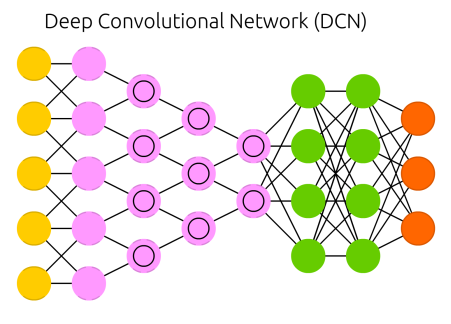
\includegraphics[width=8cm]{figuras/estrutura_c}
\caption{As redes neurais convolucionais.\footnote{Extraído de \url{https://www.asimovinstitute.org/neural-network-zoo/}}}
\label{fig:estrutura_c}
\end{figure}

Em resumo, são redes em que os neurônios de entrada não são conectados totalmente com a primeira camada oculta, mas o que acontece é que vários conjuntos distintos de neurônios da camada de entrada são conectados a várias camadas ocultas separadamente.

A seguir a união dessas camadas ocultas, exibidas como círculos rosas, conectam-se em cascata, perdendo conexões progressivamente até que um número reduzido se conecta a outras camadas, dessa vez camadas ocultas simples, que são os círculos verdes, que conectam-se em formato \eng{feedforward} até o final da rede com a camada de saída. 

Existem ainda outras dezenas de arquiteturas, algumas bem alternativas no formato e nas conexões entre as camadas, fica aqui um único exemplo dentre elas, que é a arquitetura de \defi{redes neurais extremas}. Está ilustrada na Figura \ref{fig:estrutura_e}.

\begin{figure}[htb]
\centering
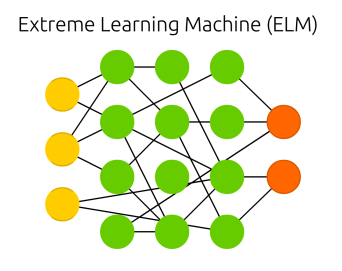
\includegraphics[width=7cm]{figuras/estrutura_e}
\caption{Redes neurais extremas.\footnote{Extraído de \url{https://www.asimovinstitute.org/neural-network-zoo/}}}
\label{fig:estrutura_e}
\end{figure}

As conexões ocorrem de forma não-sequencial, e até mesmo aleatória entre as camadas ocultas, configurando um exemplo curioso de arquitetura, e discussões mais detalhadas sobre essas outras arquiteturas não serão discutidas neste trabalho.

Este trabalho irá lidar principalmente com duas arquiteturas. Primeiramente com as redes sequenciais (ou \eng{perceptron}), numa abordagem didática, em que seu funcionamento será detalhado através de uma implementação completa dessa arquitetura no Capítulo \ref{cap:perceptron}. E a seguir, numa abordagem prática, serão utilizadas as redes convolucionais, durante os experimentos de previsões de séries temporais, no Capítulo \ref{cap:comparacao}.